\taughtsession{Lecture}{Modern Processors}{2023-12-05}{13:00}{Tamer}{}

\section{Pipelining}
Pipelining is one of the simplest, however most important, forms of \textit{Instruction Level Parallelism} (ILP). It breaks execution of instructions into a series of similar stages and organises the processor as a ``production line'', with several instructions processed \textit{concurrently} in different stages of ``production''.\\

Pipelining doesn't necessarily improve the speed of a single instruction being processed, rather it improves the \textit{throughput of the whole system}. This can be seen in the following example.\\

If we take a three stage laundry process, \textbf{W}ash, \textbf{D}ry, and \textbf{F}old, with four cycles. This can be executed sequentially as follows
\begin{verbatim}
    W-D-F-W-D-F-W-D-F-W-D-F-W-D-F
\end{verbatim}
This takes 12 cycles to complete. However, we can pipeline this instructions as follows:
\begin{verbatim}
    W-W-W-W
      D-D-D-D
        F-F-F-F
\end{verbatim}
We can see in the above example, that through pipelining the system has saved half of the processing time. Pipelining can only be utilised where each individual stage is sufficiently simple and of similar complexity to the others; this ensures that a single instruction can be executed in one clock cycle (so executed serially, it implies that it would take 4 to 5).

\subsection{How Pipelining Works in a Processor}
Shown below are the functional blocks which make up a processor. 
\begin{figure}[H]
    \centering
    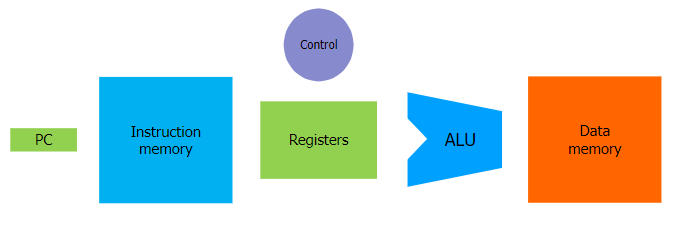
\includegraphics[width=0.9\textwidth]{assets/processor-components.png} 
    \caption{Functional blocks of a Processor}
\end{figure}
\begin{figure}[H]
    \centering
    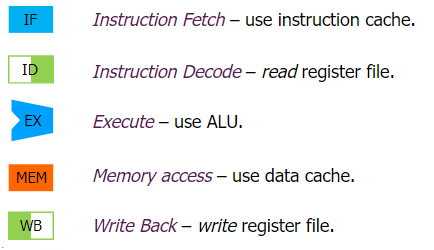
\includegraphics[width=0.6\textwidth]{assets/processor-components-functions.png}
    \caption{Processor Components Functions} 
    \label{fig:processor-components-function}
\end{figure}

As can be seen in Fig.\ref{fig:processor-components-function}, all stages of the FDE cycle operate in a different functional unit except for the ID and WB. The conflict between ID and WB is resolved by assuming that the WB writes in the first half of the cycle and ID reads in the second half. As a result of the different uses of the functional units, we have the possibility of pipelining instructions. Fig.\ref{fig:pipelining-execution-schedule} following example shows how three instructions can be pipelined to reduce the number of cycles needed to process them overall.
\begin{figure}[H]
    \centering
    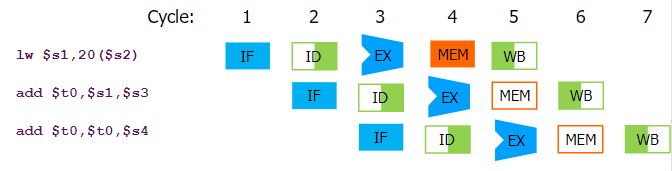
\includegraphics[width=0.9\textwidth]{assets/pipelining-execution-schedule.png}
    \caption{Execution schedule of 3 pipelined instructions}
    \label{fig:pipelining-execution-schedule}
\end{figure}

As seen above, in ideal conditions, using pipelining can create a \textit{parallel speedup} of up to 5 times. However, there are \textit{hazards} that impede this parallelism - for example dependencies between successive instructions in the pipeline. There are hardware tricks that exist to minimise the impacts of some of these, however.

\section{Superscalar Processors}
As seen in the section above, simple pipelining allows up to one instruction to be issued and completed every clock cycle. The next logical development in ILP was to issue \textit{more than one} instruction per clock cycle. This requires that processors have multiple execution units, so that more than operation of a single type (e.g. arithmetic) can be processed concurrently. Continuing with the arithmetic example - instead of a single ALU, a multiple issue processor may have a mixture of integer arithmetic units, multipliers, floating point adders, etc.\\

Executing instructions in parallel involves \textit{reordering of instructions}, which involves scheduling instructions into groups that can run together without conflicts. This can be done: in advance by the software that generates the machine code (for example Intel Itanium) or at execution time by the processor itself (for example Intel Pentium). Processors that schedule multiple instructions dynamically (at execution time) are called \textit{superscalar processors}. 

\section{Multicore and Many-Core}
Methods for increased ILP and clock speed were pursued through from the 1990s onwards, but appear to have reached their limit. In 2005, Sputter pointed out that clock speeds for Intel CPUs had stuck at around 3.5 GHz (ticks 3.5 billion times per second). Nearly twenty years on from that observation, it it still valid; clock speed is now limited by power consumption and heat dissipation.
\subsection{Multicore}
In response to a single core not performing well enough, manufacturers begun making \textit{multicore} CPUs where there are multiple independent CPUs on a single chip. Nowadays it's common to have a quad-core, hexa-core or octa-core in a consumer device; with server hardware extending to over 48-core CPUs.

\subsection{Many-Core}
In recent years, there has been a growing interest in harnessing massively parallel GPU accelerators with hundreds or thousands or processing elements for computationally demanding tasks. This is an example of a \textit{many-core} system. 